% id: 65-26
% book: 쎈B 대수 · 05 삼각함수
% section: 유형 07 부채꼴의 호의 길이와 넓이의 활용
% figure: tikz:fig-65-26
% answer: 
% answer_source: 
% variant_level: 0 (원본 전사)
% 이 파일은 build.mjs 가 items.json 에서 만든다. 고칠 때는 items.json 을 고친다.
\smash{\raisebox{4.5mm}{\dmkichul{쎈B 대수 65쪽 26번}}}
\noindent\begin{minipage}[t]{0.58\linewidth}\vspace{0pt}\raggedright 오른쪽 그림과 같은 원뿔에서 옆넓이가 밑넓이의 $\sqrt{3}$배일 때, $\cos(\angle\pt{ABO})$의 값을 구하시오.\end{minipage}\hfill\begin{minipage}[t]{0.4\linewidth}\vspace{0pt}\centering \resizebox{\ifdim\width>\linewidth\linewidth\else\width\fi}{!}{% 65-26(65쪽) — 원뿔(꼭짓점 $\pt{A}$ · 밑면의 중심 $\pt{O}$ · 밑면 둘레 위의 점 $\pt{B}$). 스캔 삽화가 흐려 TikZ 로 다시 그림.
% 라벨은 원문 것만: $\pt{A}$, $\pt{B}$, $\pt{O}$ 와 $\seg{AO}\perp\seg{BO}$ 직각 표시. 길이는 적지 않는다($\cos(\angle\pt{ABO})$ 가 읽히지 않게).
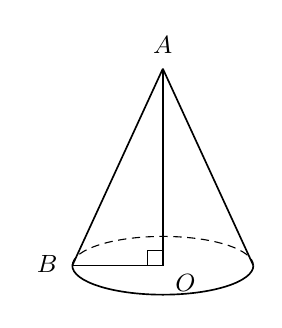
\begin{tikzpicture}[line width=0.6pt]
  \draw (0,2.5) -- (-1.15,0);
  \draw (0,2.5) -- (1.15,0);
  \draw (-1.15,0) arc (180:360:1.15 and 0.37);
  \draw[densely dashed, line width=0.4pt] (-1.15,0) arc (180:0:1.15 and 0.37);
  \draw[line width=0.5pt] (0,2.5) -- (0,0);
  \draw[line width=0.5pt] (-1.15,0) -- (0,0);
  \draw[line width=0.4pt] (-0.19,0) -- (-0.19,0.19) -- (0,0.19);
  \node[anchor=south, font=\small] at (0,2.56) {$\pt{A}$};
  \node[anchor=east, font=\small] at (-1.21,0.02) {$\pt{B}$};
  \node[anchor=north west, font=\small] at (0.03,0.02) {$\pt{O}$};
\end{tikzpicture}
}\end{minipage}\par
